
\subsection{Simulation des Grandes Échelles}

Une alternative aux deux approches précédentes est la simulation des grandes échelles, appelée Large-Eddy Simulation (LES) en anglais. Contrairement à la DNS qui résout toutes les échelles de turbulence, la LES ne représente que les grandes structures turbulentes. L'approche LES repose sur les hypothèses de similitudes de Kolmogorov [78]. Selon ces hypothèses, les grandes structures turbulentes porteuses d'énergie caractérisent l'écoulement et doivent donc être calculées, alors que le comportement des petites structures turbulentes responsables de la dissipation visqueuse peut être modélisé. En pratique, un filtre passe-bas $G$ est appliqué aux équations de Navier-Stokes pour séparer les échelles de l'écoulement qui sont calculées par les équations de celles qui sont modélisées. Les effets dissipatifs des petites échelles qui ne sont pas résolues par la LES sont pris en compte en utilisant un modèle dit "de sous-maille". Ainsi, comme la LES ne calcule pas toutes les échelles de la turbulence, le nombre de points nécessaire dans le maillage est moins important par rapport à une DNS. Pour une turbulence isotrope dans une boîte de volume égal à $L^{3}$, il varie en fonction du nombre de Reynolds comme $R e_{L}^{3 / 2}$ [6]. La LES permet donc de considérer des écoulements à des nombres de Reynolds plus élevés que la DNS, de l'ordre de $R e_{D}=10^{5}$ pour les jets simples flux [16, 25]. En revanche, compte tenu des ressources de calcul disponibles, la LES reste hors d'atteinte pour les écoulements de jets double-flux installés à $R e_{D}=10^{6}$ considérés dans chapitre 1. Simulations du bruit des jets

l'industrie. Les développements numériques réalisés dans cette thèse visent à rendre réalisable la LES pour de tels écoulements.

\begin{figure}[h!]
 \centering
 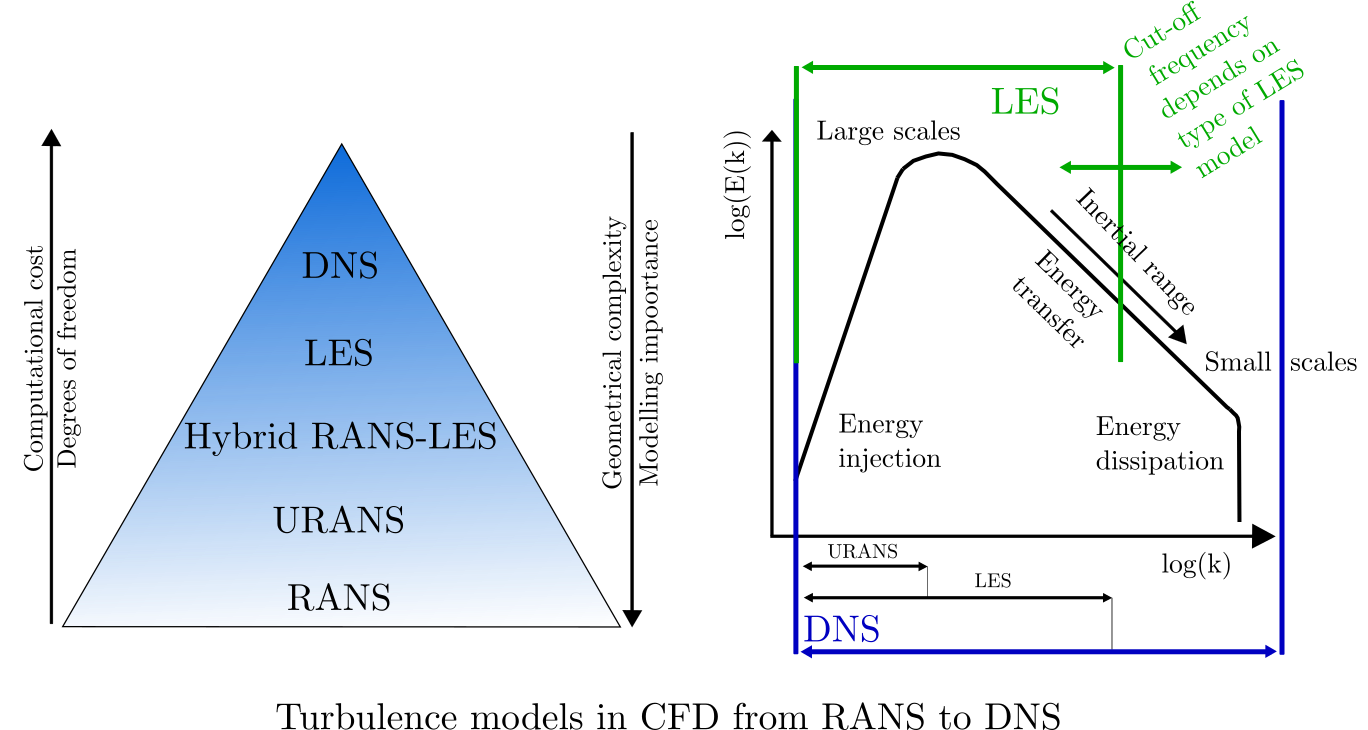
\includegraphics[width=1.0\linewidth]{chapter1_introduction/pictures/les.png}
 \vspace{-2ex}
 \caption{IXV spatial navette by esa}
  \vspace{2ex}
 \label{les}
\end{figure}
